\documentclass[11pt]{report}

%-------------------------------------------------------------------------------------------------%

% PAQUETES

\usepackage[a4paper, right = 0.8in, left = 0.8in, top = 0.8in, bottom = 0.8in]{geometry}
\usepackage[utf8]{inputenc}
\usepackage[spanish]{babel}
\usepackage{amsmath,amsfonts,amssymb,amsthm}
\usepackage{multicol}
\usepackage{fouriernc}
\usepackage{enumitem}
\usepackage{mathtools} % Solo uso \underbracket
\usepackage{cellspace, tabularx, booktabs} % Líneas del título
\usepackage{parskip}
\usepackage{pdfpages}
\usepackage{cancel}

%-------------------------------------------------------------------------------------------------%

% AJUSTES GENERALES

\setlist[enumerate]{label={\textit{\alph*})}}

\makeatletter % Para quitar el espacio adicional que el paquete parskip añade al principio y al final de una demostración
\renewenvironment{proof}[1][\proofname]{\par
  \pushQED{\qed}%
  \normalfont \topsep\z@skip % <---- changed here
  \trivlist
  \item[\hskip\labelsep
        \itshape
    #1\@addpunct{.}]\ignorespaces
}{%
  \popQED\endtrivlist\@endpefalse
}
\makeatother

%-------------------------------------------------------------------------------------------------%

% COMANDOS PERSONALIZADOS

\newcommand{\N}{\mathbb N}
\newcommand{\Z}{\mathbb Z}
\newcommand{\Q}{\mathbb Q}
\newcommand{\R}{\mathbb R}
\newcommand{\C}{\mathbb C}

\newcommand{\pars}[1]{\left( #1 \right)} % Paréntesis de tamaño automático
\newcommand{\comment}[1]{}

%-------------------------------------------------------------------------------------------------%

% EJERCICIOS Y SOLUCIONES

\newtheorem{ejercicio}{Ejercicio}
\addto\captionsspanish{\renewcommand*{\proofname}{Solución}}

%-------------------------------------------------------------------------------------------------%

\begin{document}

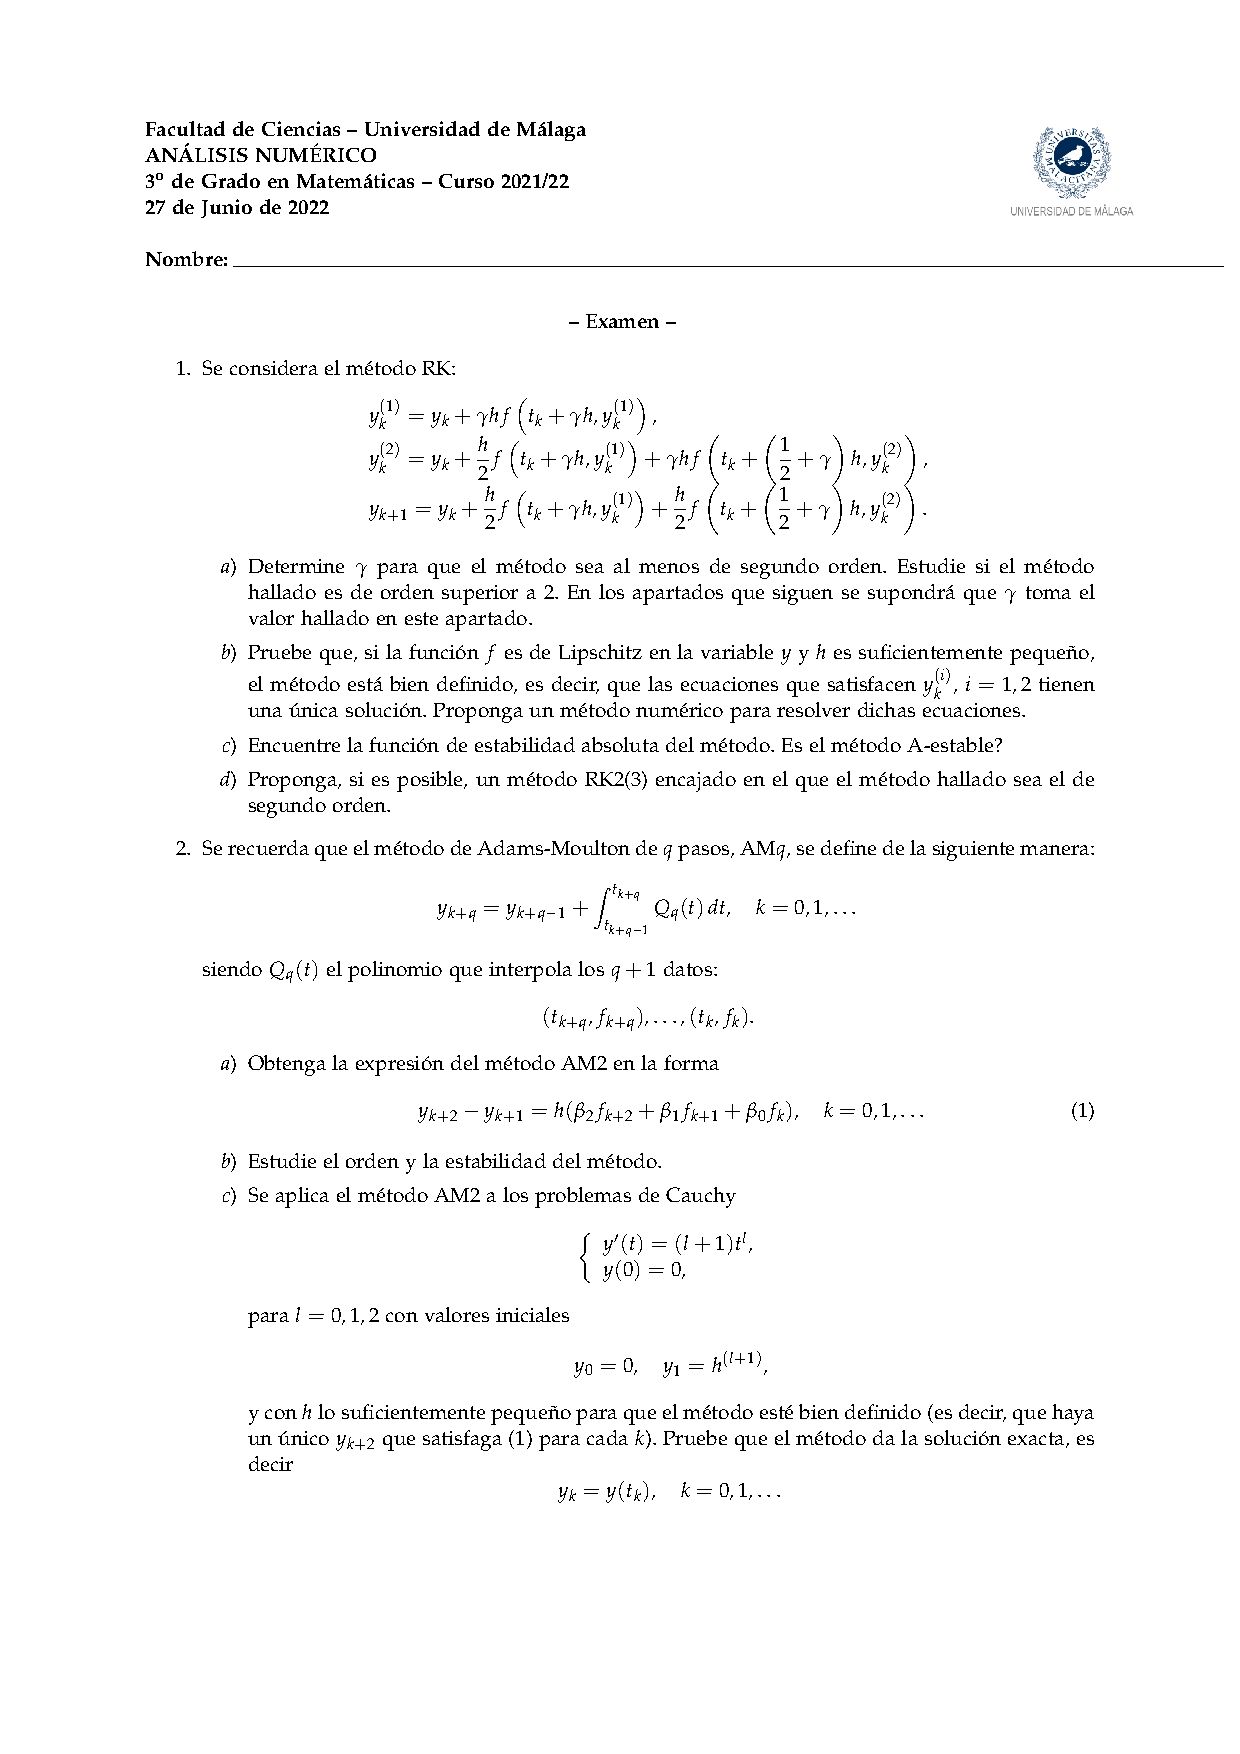
\includepdf[pages=-]{an_examen_2022-06.pdf}

%-------------------------------------------------------------------------------------------------%

% TÍTULO

\begin{center}

	\textbf{$-$ Resolución $-$}

\end{center}

%-------------------------------------------------------------------------------------------------%

\textbf{1.} El tablero de Butcher del método dado es

\begin{center}
  \setlength\extrarowheight{2.5pt}
  \begin{tabular}{c|cc}
      $\gamma$ & $\gamma$ & 0 \\
      $1/2+\gamma$ & 1/2  & $\gamma$ \\ \hline
      & 1/2 & 1/2
  \end{tabular}
  \end{center}

\begin{enumerate}
  \item Sean
  \[B = \left(\begin{array}{c}
    1/2 \\
    1/2
  \end{array}\right) \qquad \qquad E = \left(\begin{array}{c}
    1 \\
    1
  \end{array}\right) \qquad \qquad A = \left(\begin{array}{cc}
    \gamma & 0 \\
    1/2 & \gamma
  \end{array}\right) \qquad \qquad C = \left(\begin{array}{cc}
    \gamma & 0 \\
    0 & 1/2+\gamma
  \end{array}\right)\]
  Se tiene que
  \[B^tE = \left(\begin{array}{cc}
    1/2 & 1/2
  \end{array}\right)\left(\begin{array}{c}
    1 \\
    1
  \end{array}\right) = 1,\]
  así que el método es de orden $1$. De hecho,
  \[B^tAE = \left(\begin{array}{cc}
    1/2 & 1/2
  \end{array}\right)\left(\begin{array}{cc}
    \gamma & 0 \\
    1/2 & \gamma
  \end{array}\right)\left(\begin{array}{c}
    1 \\
    1
  \end{array}\right) = \left(\begin{array}{cc}
    \gamma/2+1/4 & \gamma/2
  \end{array}\right)\left(\begin{array}{c}
    1 \\
    1
  \end{array}\right) = \gamma +\frac{1}{4}\]
  El método es de orden $2$ si y solo si $\gamma +\frac{1}{4}=\frac{1}{2}$, o sea, si y solo si $\gamma = \frac{1}{4}$. Veamos si para $\gamma=\frac{1}{4}$ el método es de orden 3. Se tiene
  \[B^tC^2E = \left(\begin{array}{cc}
    1/2 & 1/2
  \end{array}\right)\left(\begin{array}{cc}
    1/4 & 0 \\
    0 & 3/4
  \end{array}\right)\left(\begin{array}{cc}
    1/4 & 0 \\
    0 & 3/4
  \end{array}\right)\left(\begin{array}{c}
    1 \\
    1
  \end{array}\right) = \left(\begin{array}{cc}
    1/8 & 3/8
  \end{array}\right)\left(\begin{array}{c}
    1/4 \\
    3/4
  \end{array}\right) = \frac{1}{32}+\frac{9}{32} = \frac{5}{16} \neq \frac{1}{3}\]
  Por tanto, el método es de orden $2$ si y solo si $\gamma = \frac{1}{4}$, y en ese caso no es de orden $3$.
  \item El sistema formado por las ecuaciones que satisfacen $y_k^{(i)}$, $i=1,2$ tiene solución única si y solo si la aplicación $G \colon \R^2 \to \R^2$ dada por 
  \[G(Y)=G\left(\begin{array}{c}
    y^1 \\
    y^2
  \end{array}\right)=\left(\begin{array}{c}
    y_k+\frac{h}{4}f(t_k+\frac{h}{4},y^1) \\[5pt]
    y_k+\frac{h}{2}f(t_k+\frac{h}{4},y^1)+\frac{h}{4}f(t_k+\frac{3h}{4},y^2)
  \end{array}\right)\]
  tiene un único punto fijo. Veamos cómo de pequeño debe ser $h$ para que se tenga la contractividad de $G$. Si $Y,Z \in \R^2$,
  \[
  \begin{aligned}[t]
     |G_1(Y)-G_1(Z)| &= \bigl|y_k+\frac{h}{4}f\bigl(t_k+\frac{h}{4},y^1\bigr) -y_k-\frac{h}{4}f\bigl(t_k+\frac{h}{4},z^1\bigr) \bigr| = \frac{h}{4}\bigl|f\bigl(t_k+\frac{h}{4},y^1\bigr)-f\bigl(t_k+\frac{h}{4},z^1\bigr)\bigr| \\
     &\leq \frac{hL}{4} |y^1-z^1| \leq \frac{hL}{4} ||Y-Z||_{\infty},
  \end{aligned}
  \]
  donde $L$ es la constante de Lipschitz de $f$. Además,
  \[
  \begin{aligned}[t]
     |G_2(Y)-G_2(Z)| &= \bigl|y_k+\frac{h}{2}f\bigl(t_k+\frac{h}{4},y^1\bigr)+\frac{h}{4}f\bigl(t_k+\frac{3h}{4},y^2\bigr)-y_k-\frac{h}{2}f\bigl(t_k+\frac{h}{4},z^1\bigr)-\frac{h}{4}f\bigl(t_k+\frac{3h}{4},z^2\bigr) \bigr|  \\
     &\leq \frac{h}{2}\bigl|f\bigl(t_k+\frac{h}{4},y^1\bigr)-f\bigl(t_k+\frac{h}{4},z^1\bigr)\bigr|+\frac{h}{4}\bigl|f\bigl(t_k+\frac{3h}{4},y^2\bigr)-f\bigl(t_k+\frac{3h}{4},z^2\bigr)\bigr| \\
     &\leq \frac{hL}{2}|y^1-z^1|+\frac{hL}{4}|y^2-z^2| \leq \frac{3hL}{4} ||Y-Z||_{\infty}
  \end{aligned}
  \]
  Por tanto,
  \[||G(Y)-G(Z)||_{\infty} \leq \frac{3hL}{4}||Y-Z||_\infty\]
  Si tomamos $h$ de forma que
  \[0<h<\frac{4}{3L}\]
  entonces se tendrá $0<\frac{3hL}{4}<1$, así que $G$ será contractiva y el teorema del punto fijo de Banach dirá que $G$ tiene un único punto fijo, que es la única solución del sistema del método RK. Es más, el teorema de Banach también dice que la sucesión dada por
  \[\begin{cases}
    Y_0 \in \R^2 \\
    Y_{n+1} = G(Y_n), \qquad n = 0,1,\mathellipsis
  \end{cases}\]
  converge al único punto fijo de $G$, así que este algoritmo de punto fijo es un buen método numérico para resolver las ecuaciones.
  \item La función de estabilidad absoluta del método es 
  \[\begin{aligned}[t]
    R(\hat{h}) &= \frac{|I-\hat{h}A+hEB^t|}{|I-\hat{h}A|} = \left|\begin{array}{cc}
      1 - \hat{h}/4 & 0 \\
      -\hat{h}/2 & 1-\hat{h}/4 
    \end{array} \right|^{-1}\left|\begin{array}{cc}
      1 - \hat{h}/4+\hat{h}/2 & \hat{h}/2 \\
      -\hat{h}/2+\hat{h}/2 & 1-\hat{h}/4 +\hat{h}/2
    \end{array}\right| \\ &= \left|\begin{array}{cc}
      1 - \hat{h}/4 & 0 \\
      -\hat{h}/2 & 1-\hat{h}/4 
    \end{array} \right|^{-1}\left|\begin{array}{cc}
      1 + \hat{h}/4 & \hat{h}/2 \\
      0 & 1+\hat{h}/4
    \end{array}\right| = \frac{(1+\hat{h}/4)^2}{(1-\hat{h}/4)^2} = \frac{(4+\hat{h})^2}{(4-\hat{h})^2}
  \end{aligned}  \]
  Sea $\hat{h}=x+iy \in \C^-$. Entonces
  \[\begin{aligned}[t]
      |R(\hat{h})| < 1 \iff |4+\hat{h}|^2 < |4-\hat{h}|^2 \iff (4+x)^2+y^2 < (4-x)^2+y^2 \iff 16+x^2+8x < 16+x^2-8x
  \end{aligned}\]
  Esto último es siempre cierto por ser $x<0$, así que $\C^- \subset D_A$ y por tanto el método es $A$-estable.
  \item No entra.
\end{enumerate}

\textbf{2. }

\begin{enumerate}
  \item El polinomio que interpola los datos
  \[(t_{k+2},f_{k+2}),(t_{k+1},f_{k+1}),(t_{k},f_k)\]
  es, en la forma regresiva de Gregory-Newton,
  \[Q(t)=\widetilde{Q}\left(\frac{t-t_{k+2}}{h}\right),\]
  donde
  \[
  \widetilde{Q}(s)=\sum_{j=0}^2 \nabla^jf_{k+2}\binom{s+j-1}{j} = \nabla^0f_{k+2}+s\nabla^1f_{k+2}+\frac{1}{2}(s^2+s)\nabla^2f_{k+2} \]
  Por tanto, la expresión del método AM2 es
  \[\begin{aligned}[t]
    y_{k+2} &= y_{k+1}+\int_{t_{k+1}}^{t_{k+2}}Q(t) \, dt =  y_{k+1}+\int_{t_{k+1}}^{t_{k+2}}\widetilde{Q}\left(\frac{t-t_{k+2}}{h}\right) \, dt \overset{(\ast)}{=} y_{k+1}+h\int^0_{-1}\widetilde{Q}(s) \, ds \\
    &= y_{k+1}+h\left(\nabla^0 f_{k+2}\int_{-1}^0 1 \, ds + \nabla^1f_{k+2}\int_{-1}^0 s \, ds + \frac{1}{2}\nabla^2f_{k+2}\int_{-1}^0 (s^2+s) \, ds\right) \\
    &=y_{k+1}+h\left(\nabla^0 f_{k+2}-\frac{1}{2} \nabla^1f_{k+2} + \frac{1}{2}\nabla^2f_{k+2}\left(\frac{1}{3}-\frac{1}{2}\right)\right)=y_{k+1}+h\left(\nabla^0 f_{k+2}-\frac{1}{2} \nabla^1f_{k+2} - \frac{1}{12}\nabla^2f_{k+2}\right) \\
    &=y_{k+1}+h\left(f_{k+2}-\frac{1}{2} (f_{k+2}-f_{k+1}) - \frac{1}{12}(f_{k+2}-2f_{k+1}+f_k)\right) \\
    &= y_{k+1}+h\left(f_{k+2}-\frac{1}{2} (f_{k+2}-f_{k+1}) - \frac{1}{12}(f_{k+2}-2f_{k+1}+f_k)\right) \\
    &= y_{k+1}+h\left(\frac{5}{12}f_{k+2}+\frac{2}{3}f_{k+1}-\frac{1}{12}f_k\right)
  \end{aligned}\]
  En $(\ast)$ se ha realizado el cambio de variable $t = sh+t_{k+2}$, $dt = h \, ds$.
  \item El primer polinomio característico del método es $\rho(z)=z^2-z = z(z-1)$, cuyas raíces son de módulo menor que $1$ y la que es de módulo $1$ es simple. Por tanto, el método es estable. Estudiemos el orden. En primer lugar,
  \[\sum_{j=0}^2 \alpha_j = 1-1 = 0\]
  Además,
  \[\sum_{j=0}^2 \alpha_jj = -1+2 = 1, \qquad \qquad \sum_{j=0}^2 \beta_j = \frac{5}{12}+\frac{8}{12}-\frac{1}{12} = 1,\]
  luego el método es de orden $1$. Más cuentas:
  \[\sum_{j=0}^2 \alpha_jj^2 = -1+4 = 3, \qquad \qquad 2\sum_{j=0}^2 \beta_jj = 2\left(2 \cdot \frac{5}{12}+\frac{8}{12}\right) = \frac{36}{12} = 3\]
  Por tanto, el método es de orden $2$. De hecho
  \[\sum_{j=0}^2\alpha_jj^3 = -1+8 = 7, \qquad \qquad 3\sum_{j=0}^2 \beta_jj^2 = 3\left(4\cdot \frac{5}{12}+\frac{8}{12}\right) = \frac{3 \cdot 28}{12} = \frac{28}{4} = 7,\]
  y entonces el método es de orden $3$. Sin embargo,
  \[\sum_{j=0}^2 \alpha_jj^4 = -1+16 = 15, \qquad \qquad 4\sum_{j=0}^2 \beta_jj^3 = 4\left(8\cdot \frac{5}{12}+\frac{8}{12}\right) = \frac{4 \cdot 48}{12} = \frac{48}{3} = 16,\]
  así que el método no es de orden $4$.
  \item Sea $f(t,y)=(l+1)t^l$. El método AM2 para este problema es 
  \[
  \begin{aligned}[t]
    y_{k+2}&=y_{k+1}+h\left(\frac{5}{12}(l+1)t_{k+2}^l+\frac{2}{3}(l+1)t_{k+1}^l -\frac{1}{12}(l+1)t_k^l\right) \\ &= y_{k+1}+h^{l+1}(l+1)\left(\frac{5}{12}(k+2)^l+\frac{2}{3}(k+1)^l -\frac{1}{12}k^l\right)
  \end{aligned}
  \]
  La solución exacta del problema es $y(t)=t^{l+1}$. Veamos que para $l=0,1,2$ el método da la solución exacta. Si $l = 0$, entonces $y(t)=t$, $y_1 = h$ y el método adopta la expresión
  \[y_{k+2}=y_{k+1}+h\left(\frac{5}{12}+\frac{2}{3} -\frac{1}{12}\right) = y_{k+1}+h\]
  Razonando por recurrencia,
  \[y_k = y_{k-1}+h = y_{k-2}+2h = \mathellipsis = y_1+(k-1)h =  h+(k-1)h = kh = y(kh) = y(t_k),\]
  luego el método da la solución exacta. Si $l = 1$, entonces $y(t)=t^2$, $y_1 = h^2$ y el método adopta la expresión
  \[\begin{aligned}[t]
    y_{k+2}=y_{k+1}+2h^2\left(\frac{5}{12}(k+2)+\frac{2}{3}(k+1)-\frac{1}{12}k\right) = y_{k+1}+2h^2\left(k +\frac{10}{12}+\frac{8}{12}\right) = y_{k+1}+2h^2\left(k +\frac{3}{2}\right)
  \end{aligned}
    \]
  Razonando por recurrencia,
  \[
  \begin{aligned}[t]
    y_k &= y_{k-1}+2h^2\left(k-2+\frac{3}{2}\right) =  y_{k-1}+2h^2\left(k-\frac{1}{2}\right) = y_{k-2}+2h^2\left(k-1-\frac{1}{2} \right)+2h^2\left(k-\frac{1}{2}\right) \\
    &= y_{k-2}+2h^2\left(k+(k-1)-\frac{2}{2}\right) = \mathellipsis = y_1+2h^2\left(\sum_{i=2}^k i -\frac{k-1}{2}\right) = h^2+2h^2\left(\frac{k(k+1)}{2}-1 -\frac{k-1}{2}\right) \\
    &=  h^2+2h^2\left(\frac{k^2}{2}+\frac{k}{2}-1-\frac{k}{2}+\frac{1}{2}\right) =  h^2+2h^2\left(\frac{k^2}{2}-\frac{1}{2}\right) = h^2+h^2k^2-h^2 = h^2k^2 = y(kh) = y(t_k),
  \end{aligned}
 \]
 luego el método da la solución exacta. Para $l = 2$ es altamente probable que las cuentas sean muy desagradables.
\end{enumerate}

\textbf{3. }

\begin{enumerate}
  \item  Para cada $i \in \{0,1,\mathellipsis,N+1\}$, sea $u_i$ la aproximación de $y(x_i)$. Evidentente, tomamos $u_{N+1}=1$ porque $y(x_{N+1})=y(1)=1$. Para $i =1,2,\mathellipsis,N$, se realizan las aproximaciones
  \[y''(x_i) \approx \frac{y(x_{i+1})-2y(x_i)+y_{x-i}}{h^2}, \qquad \qquad y'(x_i) \approx \frac{y(x_{i+1})-y(x_{i-1})}{2h},\]
  es decir,
  \[y''(x_i) \approx \frac{u_{i+1}-2u_i+u_{i-1}}{h^2}, \qquad \qquad y'(x_i) \approx \frac{u_{i+1}-u_{i-1}}{2h}\]
  Sustituyendo en la ecuación del problema, debe cumplirse
  \[\frac{u_{i+1}-2u_i+u_{i-1}}{h^2} + \frac{u_{i+1}-u_{i-1}}{2h} + u_i^2 = x_i^3, \qquad i =1,2,\mathellipsis,N-1 \tag{$\ast$}\]
  Para $i = N$, usando que $u_{N+1} = 1$,
  \[\frac{1-2u_N+u_{N-1}}{h^2} + \frac{1-u_{N-1}}{2h} + u_N^2 = x_N^3\]
  Esto proporciona un sistema de $N$ ecuaciones con $N+1$ incógnitas, $u_0,u_1,\mathellipsis,u_N$ ($u_{N+1}$ no es una incógnita), así que hay que añadir una ecuación más que trate la condición de contorno en $x_0$. Para $i = 0$, consideramos un nodo fantasma $u_{-1}$ para aproximar $y'(x_0)$:
  \[y'(x_0) \approx \frac{u_1-u_{-1}}{2h}\]
  Como $y'(x_0) = y'(0)=1$, entonces debe cumplirse
  \[\frac{u_1-u_{-1}}{2h} = 1\]
  Por tanto,
  \[u_{-1} = 2h-u_1\]
  y sustituyendo en $(\ast)$ para $i = 0$ tendríamos
  \[\frac{u_{1}-2u_0+2h-u_1}{h^2} + \frac{u_{1}-2h-u_1}{2h} + u_0^2 = 0,\]
  es decir,
  \[\frac{-2u_0+2h}{h^2} -1 + u_0^2 = 0\]
  Uniendo esta ecuación con las $N+1$ anteriores ya se dispone de un sistema de $N+1$ ecuaciones con $N+1$ incógnitas cuya solución (en caso de haberla) proporciona una aproximación de la solución del problema de partida:
  \[(S) \ \left\{ \begin{alignedat}{1}
    \frac{-2u_0+2h}{h^2} -1 + u_0^2 &= 0 \\
    \frac{u_{i+1}-2u_i+u_{i-1}}{h^2} + \frac{u_{i+1}-u_{i-1}}{2h} + u_i^2 &= x_i^3, \qquad i =1,2,\mathellipsis,N-1 \\
    \frac{1-2u_N+u_{N-1}}{h^2} + \frac{1-u_{N-1}}{2h} + u_N^2 &= x_N^3
  \end{alignedat} \right.\]
  \item Resolver el sistema $(S)$ es lo mismo que encontrar los ceros de la función $\Phi \colon \R^{N+1} \to \R^{N+1}$ dada por
  \[\Phi(U) = \Phi\left(\begin{array}{c}
    u_0 \\
    u_1 \\
    \vdots \\
    u_{N-1} \\
    u_N
  \end{array}\right) = \left(\begin{array}{c}
    \frac{-2u_0+2h}{h^2}-1+u_0^2 \\[5pt]
    \frac{u_{2}-2u_1+u_{0}}{h^2} + \frac{u_{2}-u_{0}}{2h} + u_1^2 - x_1^3 \\[5pt]
    \vdots \\
    \frac{u_{N}-2u_{N-1}+u_{N-2}}{h^2} + \frac{u_N-u_{N-2}}{2h} + u_{N-1}^2 - x_{N-1}^3 \\[5pt]
    \frac{1-2u_N+u_{N-1}}{h^2} + \frac{1-u_{N-1}}{2h} + u_N^2 - x_N^3
  \end{array}\right)\]
  \item El método de Newton para la resolución del sistema no lineal $\Phi(U)=0$ es
  \[U_{n+1} = U_{n}-J(U_n)^{-1}\Phi(U_n), \qquad n = 0,1,2,\mathellipsis\]
  donde
  \[J(U_n) = \left(\begin{array}{cccc}
    \frac{\partial \Phi_0}{\partial u_0} & \frac{\partial \Phi_0}{\partial u_1} & \mathellipsis & \frac{\partial \Phi_0}{\partial u_N} \\[5pt]
    \frac{\partial \Phi_1}{\partial u_0} & \frac{\partial \Phi_1}{\partial u_1} & \mathellipsis & \frac{\partial \Phi_1}{\partial u_N} \\[5pt]
    \vdots & \vdots & \ddots & \vdots \\[5pt]
    \frac{\partial \Phi_N}{\partial u_0} & \frac{\partial \Phi_N}{\partial u_1} & \mathellipsis & \frac{\partial \Phi_N}{\partial u_N}
  \end{array}\right)
  \]
  Se tiene que
  \[U_{n+1} = U_{n}-J(U_n)^{-1}\Phi(U_n) \iff J(U_n)(U_{n}-U_{n+1}) = \Phi(U_n) \iff \begin{cases}
    J(U_n)V_n = \Phi(U_n) \\
    U_{n+1} = U_n-V_n
  \end{cases}\]
  De esta manera, evitamos el cálculo de la matriz inversa de $J(U_n)$ y el método de Newton se reduce a resolver un sistema lineal en cada iteración, con matriz de coeficientes
  \[J(U_n) = \left(\begin{array}{cccccc}
      -\frac{2}{h^2}+2u_0 & 0 & 0 & 0 & \mathellipsis & 0 \\[5pt]
      \frac{1}{h^2}-\frac{1}{2h} & -\frac{2}{h^2}+2u_1 & \frac{1}{h^2} + \frac{1}{2h} & 0 & \mathellipsis & 0 \\[5pt]
      0 & \frac{1}{h^2}-\frac{1}{2h} & -\frac{2}{h^2}+2u_2 & \frac{1}{h^2} + \frac{1}{2h} & \mathellipsis & 0 \\
      \vdots & \vdots & \vdots & \vdots & \ddots & \vdots \\
      0 & 0 & 0 & 0 & \mathellipsis & -\frac{2}{h^2}+2u_N
  \end{array}\right)\]
  y vector de términos independientes $\Phi(U_n)$, que ya ha sido detallado antes.
\end{enumerate}

\end{document}